\begin{frame}[t,fragile] \frametitle{Nascita della AI}
	{\scriptsize
		\onslide<1->
            \framesubtitle{Il primo programma informatico della storia}
            \vspace*{-15pt}
             \begin{minipage}[t]{\textwidth}
             	\begin{figure}[ht]
                    \centering
                    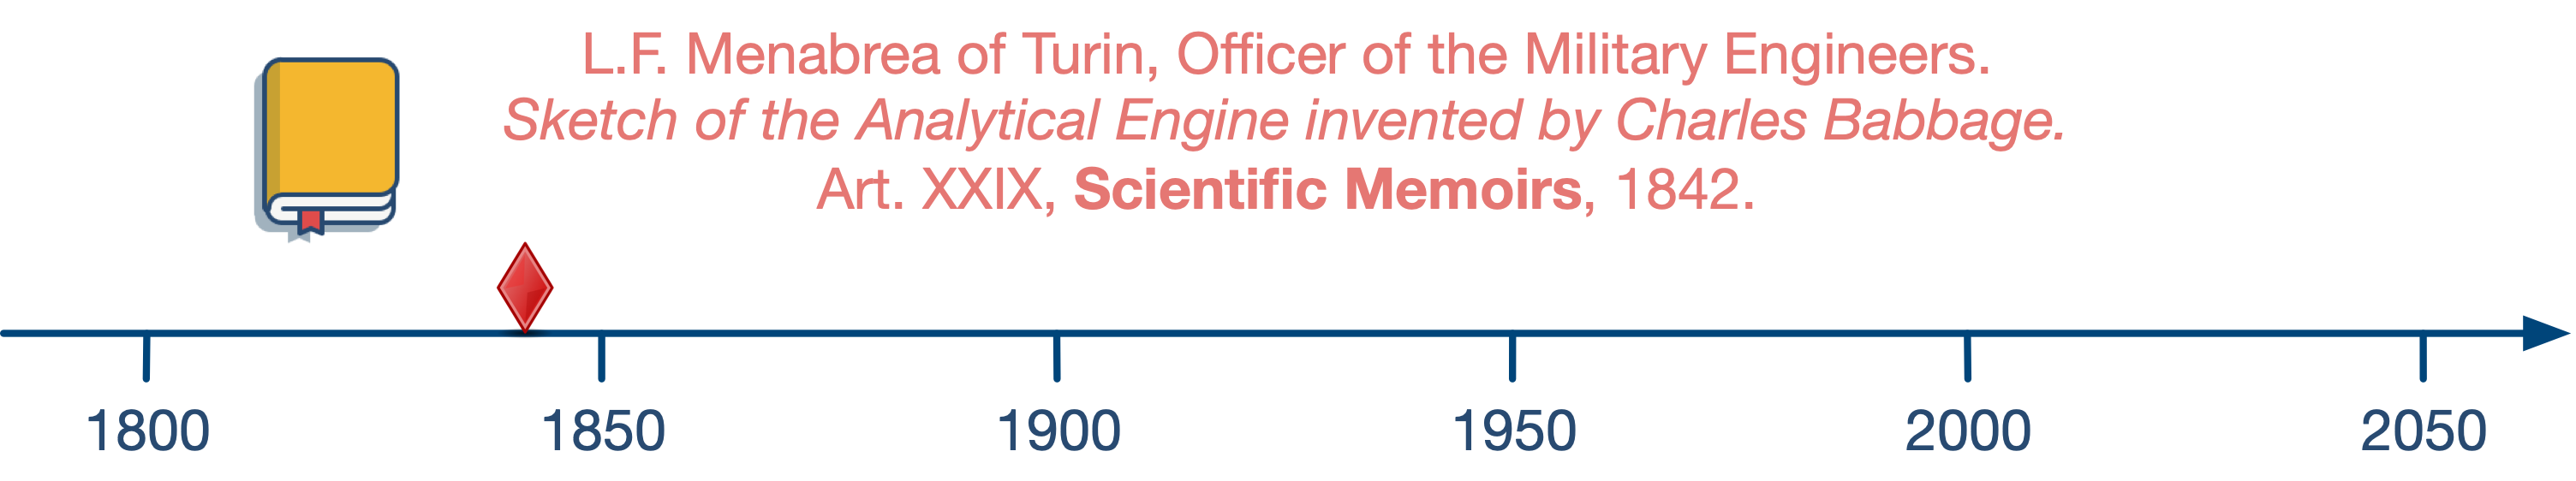
\includegraphics[width=\textwidth]{img/AI-timeline-1842-alt.png}
                \end{figure}
            \end{minipage}
            \\\vspace*{3pt}
	    	\begin{minipage}[t]{\textwidth}
				\begin{minipage}[t]{0.6\textwidth}
	    			\begin{itemize}[leftmargin=10pt,align=right]
						\onslide<2->\item[\alert{\faHandORight}] Mente visionaria dietro la \alert{macchina analitica di Babbage}
						\onslide<3->\item[\alert{\faHandORight}] Definì per prima il concetto di \alert{ricorsione algoritmica} nel caso della computazione dei numeri di Bernoulli
						\onslide<4->\item[\alert{\faHandORight}] Contributo dimostrato solo un secolo dopo (Harvard Mark I ideato da Howard Aiken e finanziato da IBM nel 1944)
						\onslide<5->\item[\alert{\faHandORight}] Macchina di calcolo che si potesse programmare e riprogrammare per eseguire diverse funzioni (\alert{macchina universale})
					\end{itemize}
            	\end{minipage}
            	%
				\onslide<1->
            	\begin{minipage}[t]{0.4\textwidth}
                	\centering
                	\begin{figure}[ht]
                    	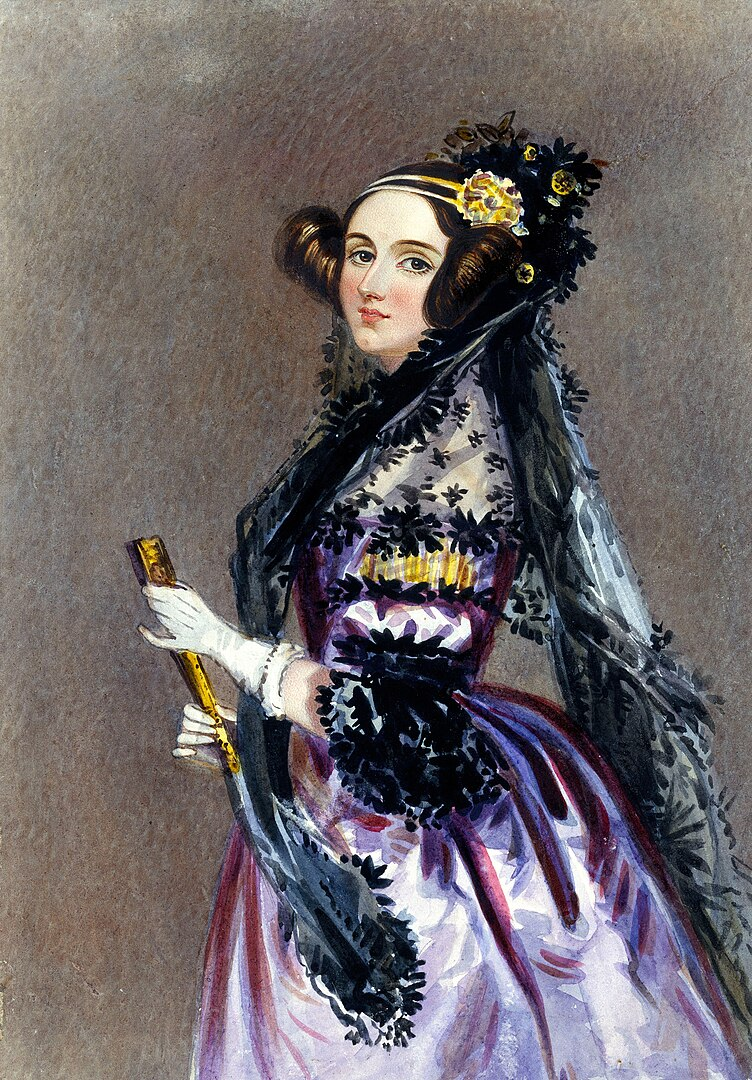
\includegraphics[width=.6\textwidth]{752px-Ada_Lovelace_portrait.jpg}
                    	{\tiny\\Augusta Ada Byron Lovelace\\\vspace*{-1pt}\textit{\textcopyright Wikimedia Creative Commons}}
                	\end{figure}
            	\end{minipage}
	    	\end{minipage}
	}
\end{frame}
%
\begin{frame}[t,fragile] \frametitle{Nascita della AI}
	{\scriptsize
		\onslide<1->
            \framesubtitle{Dalla macchina al \textit{test} di Turing}
            \vspace*{-15pt}
            \begin{minipage}[t]{\textwidth}
             	\begin{figure}[ht]
                    \centering
                    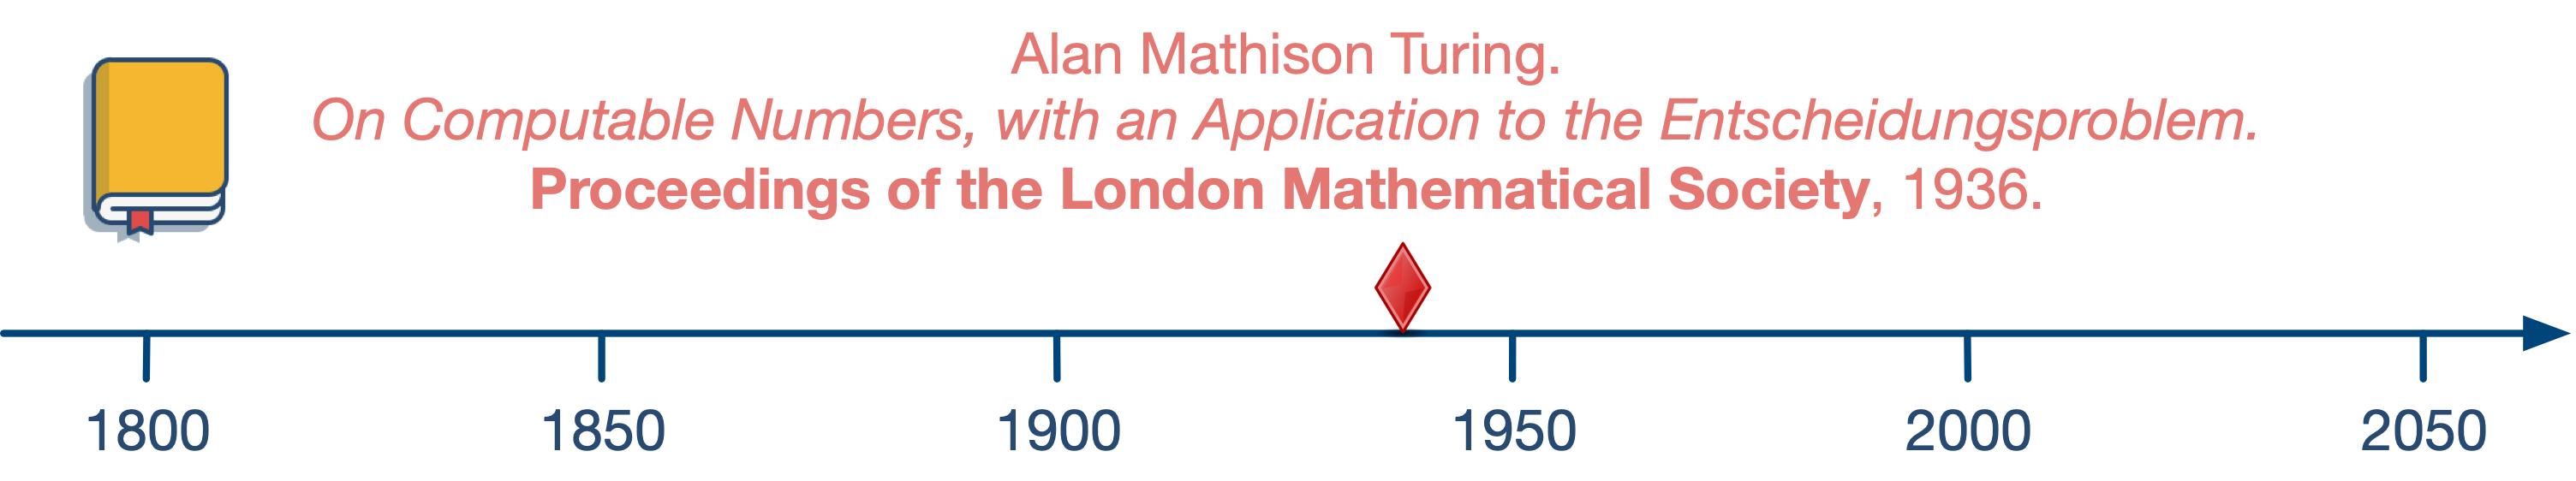
\includegraphics[width=\textwidth]{img/AI-timeline-1936-alt.png}
                \end{figure}
            \end{minipage}
            \\\vspace*{3pt}
	    	\begin{minipage}[t]{\textwidth}
				\begin{minipage}[t]{0.6\textwidth}
	    			\begin{itemize}[leftmargin=10pt,align=right]
						\onslide<2->\item[\alert{\faHandORight}] Modello di calcolo astratto in grado di eseguire sequenze di istruzioni (\alert{algoritmi}) attraverso lettura e scrittura su nastro e regole (simulazione del processo di calcolo umano)
						\onslide<3->\item[\alert{\faHandORight}] Ogni funzione computabile è Turing-computabile
                    	\onslide<4->\begin{itemize}[leftmargin=10pt,align=right]
							\item[\alert{\faHandORight}] Tutto ciò che una macchina di calcolo reale può computare è calcolabile da una macchina di Turing
							\item[\alert{\faHandORight}] \textit{Standard} per definire la complessità di un algoritmo, la decidibilità o meno di un problema da risolvere
						\end{itemize}
                    	\onslide<5->\item[\alert{\faHandORight}] Ultimo \alert{\textbf{no}} al \alert{problema della decidibilità} di Hilbert (1928)
						\begin{itemize}[leftmargin=10pt,align=right]
							\item[\alert{\faHandORight}] \textit{Esiste una procedura meccanica in grado di decidere in tempo finito se, nell'ambito di una teoria matematica, una data affermazione sia vera o falsa?}
						\end{itemize}
					\end{itemize}
            	\end{minipage}
				%
				\onslide<1->
            	\begin{minipage}[t]{0.4\textwidth}
                	\centering
                	\begin{figure}[ht]
						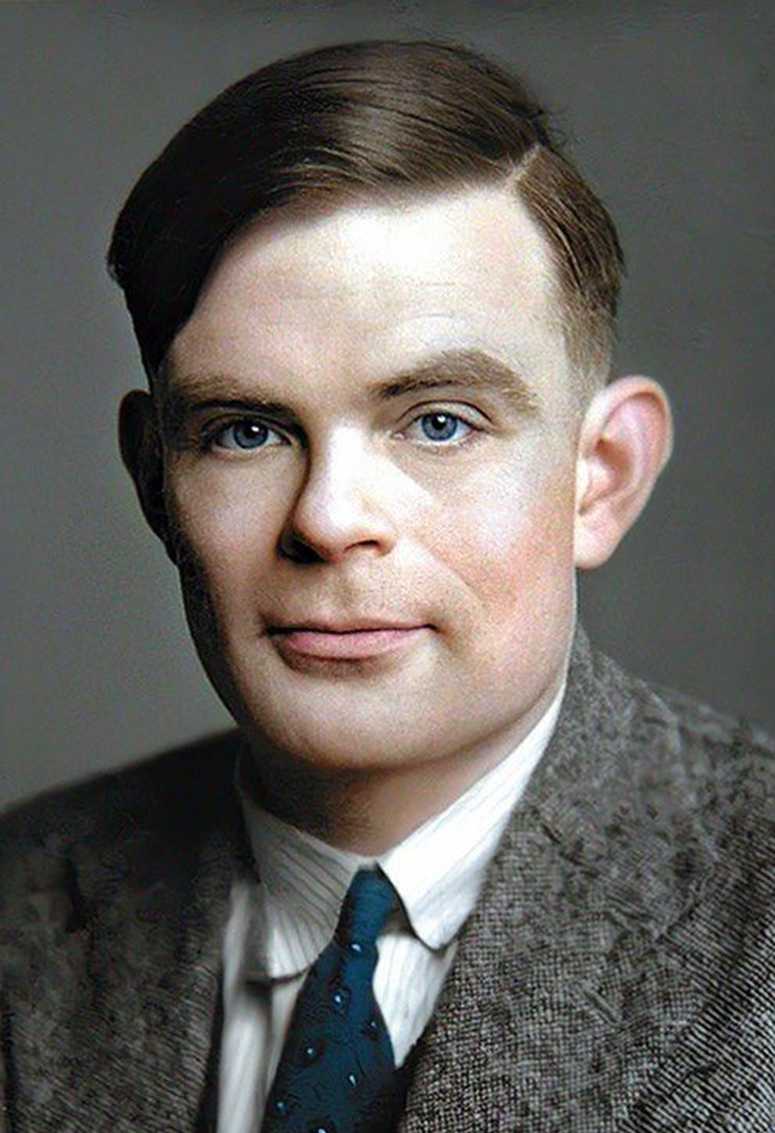
\includegraphics[width=.6\textwidth]{img/alan-turing-color.png}
						{\tiny\\Alan Mathison Turing\\\vspace*{-1pt}\textit{\textcopyright Elcorreo.com}}
                	\end{figure}
            	\end{minipage}
	    	\end{minipage}
	}
\end{frame}
%
\begin{frame}[t,fragile] \frametitle{Nascita della AI}
    {\scriptsize
    \onslide<1->
        \framesubtitle{Dalla macchina al \textit{test} di Turing}
        \vspace*{-15pt}
	    \begin{minipage}[t]{\textwidth}
		    \begin{figure}[ht]
			    \centering
			    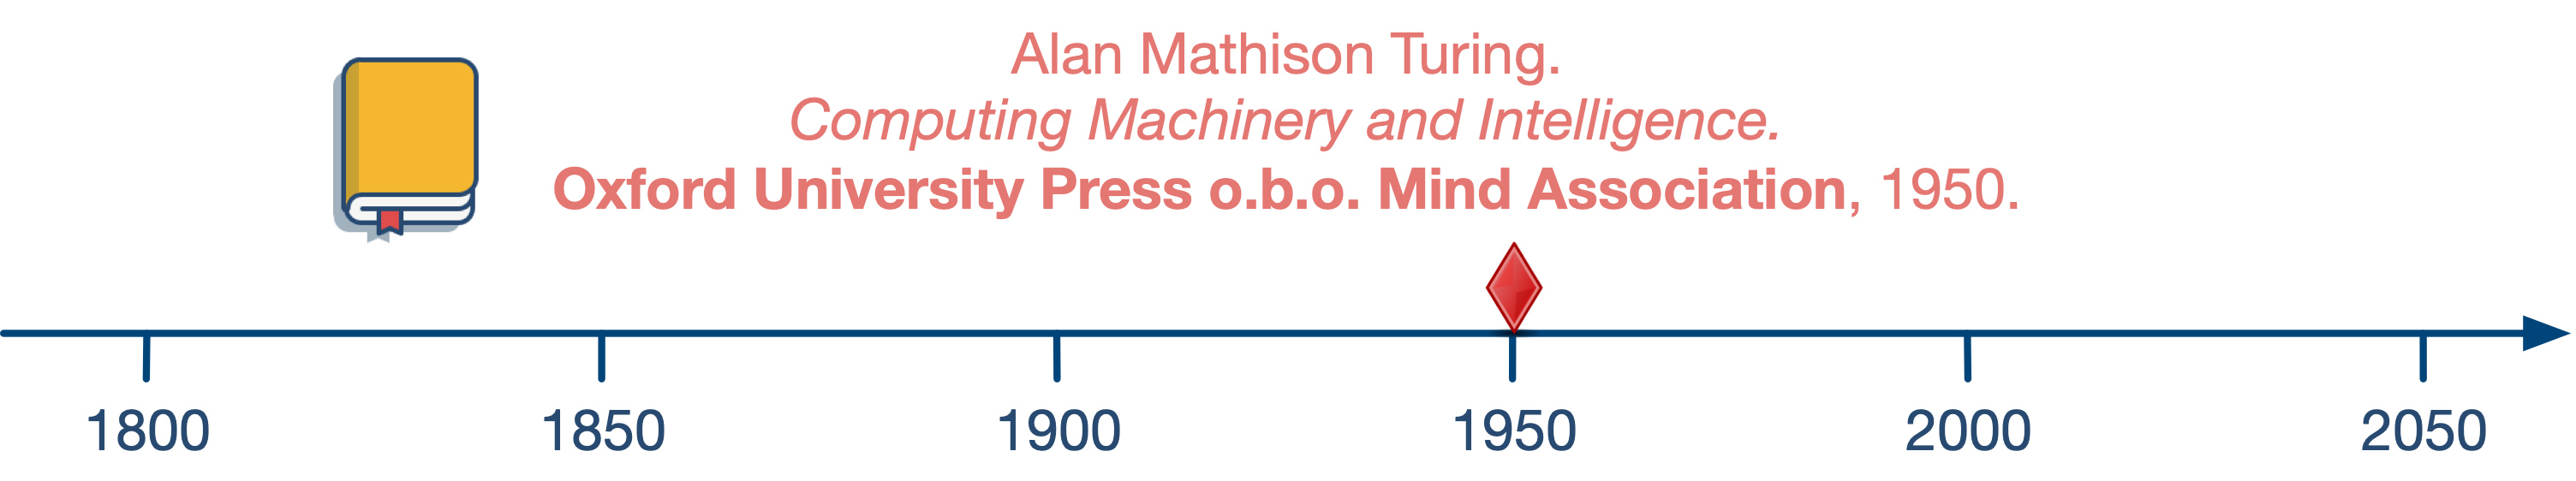
\includegraphics[width=\textwidth]{img/AI-timeline-1950-alt.png}
		    \end{figure}
	    \end{minipage}
	    \\\vspace*{3pt}
	    \begin{minipage}[t]{\textwidth}
		    \begin{minipage}[t]{0.6\textwidth}
			    \begin{itemize}[leftmargin=10pt,align=right]
				    \onslide<2->\item[\alert{\faHandORight}] Propone il primo esperimento per valutare l'intelligenza di una macchina (\alert{\textit{test} di Turing} o \alert{\textit{Imitation Game}})
				    \onslide<3->\begin{itemize}[leftmargin=10pt,align=right]
						\item[\alert{\faHandORight}] Una macchina e un umano in due stanze separate
						\item[\alert{\faHandORight}] Un arbitro umano pone delle domande a entrambi per definire chi è l'umano dei due
						\item[\alert{\faHandORight}] Se l'arbitro non riesce a determinare la natura degli interlocutori, allora la macchina ha raggiunto un comportamento intelligente
				    \end{itemize}
				    \onslide<4->\item[\alert{\faHandORight}] Impone la comprensione del linguaggio come \alert{condizione sufficiente} dell'intelligenza
			    \end{itemize}
		    \end{minipage}
		    %
		    \onslide<1->
		    \begin{minipage}[t]{0.4\textwidth}
			    \centering
			    \begin{figure}[ht]
				    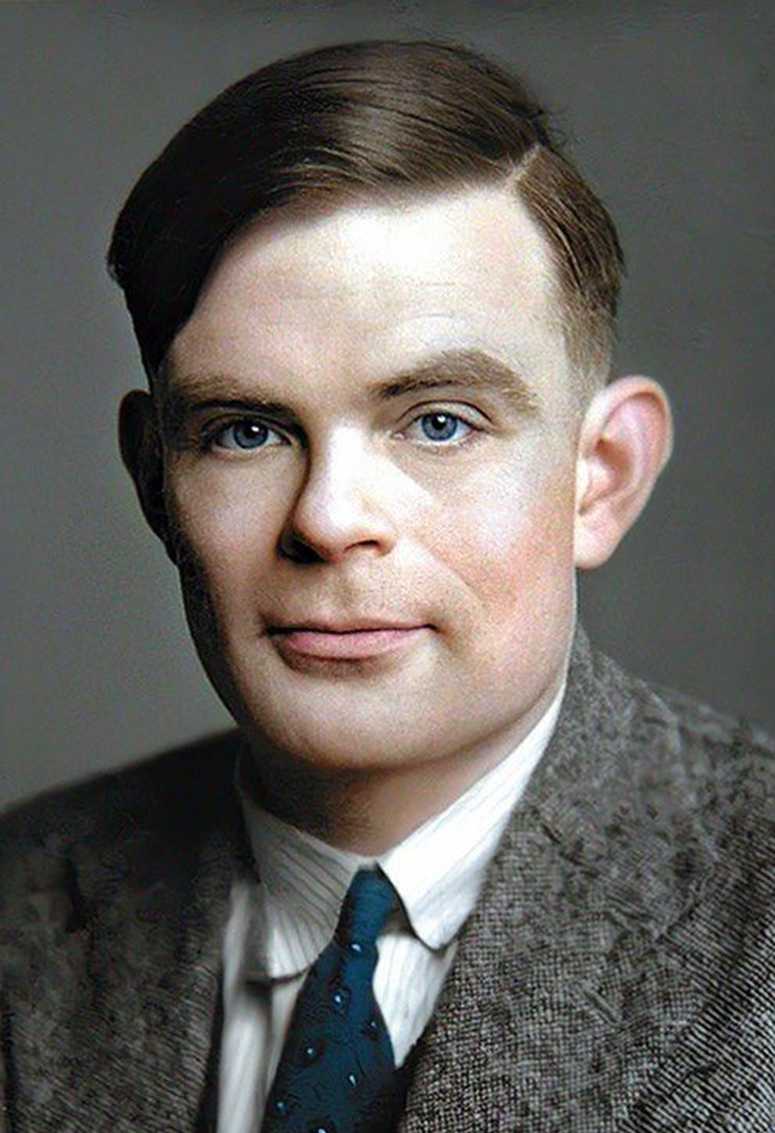
\includegraphics[width=.6\textwidth]{img/alan-turing-color.png}
				    {\tiny\\Alan Mathison Turing\\\vspace*{-1pt}\textit{\textcopyright Elcorreo.com}}
			    \end{figure}
		    \end{minipage}
	    \end{minipage}
    }
\end{frame}
%
\begin{frame}[t,fragile] \frametitle{Nascita della AI}
{\scriptsize
	\onslide<1->
		\framesubtitle{\textit{Habemus} AI!}
		\vspace*{-15pt}
		\begin{minipage}[t]{\textwidth}
			\begin{figure}[ht]
				\centering
				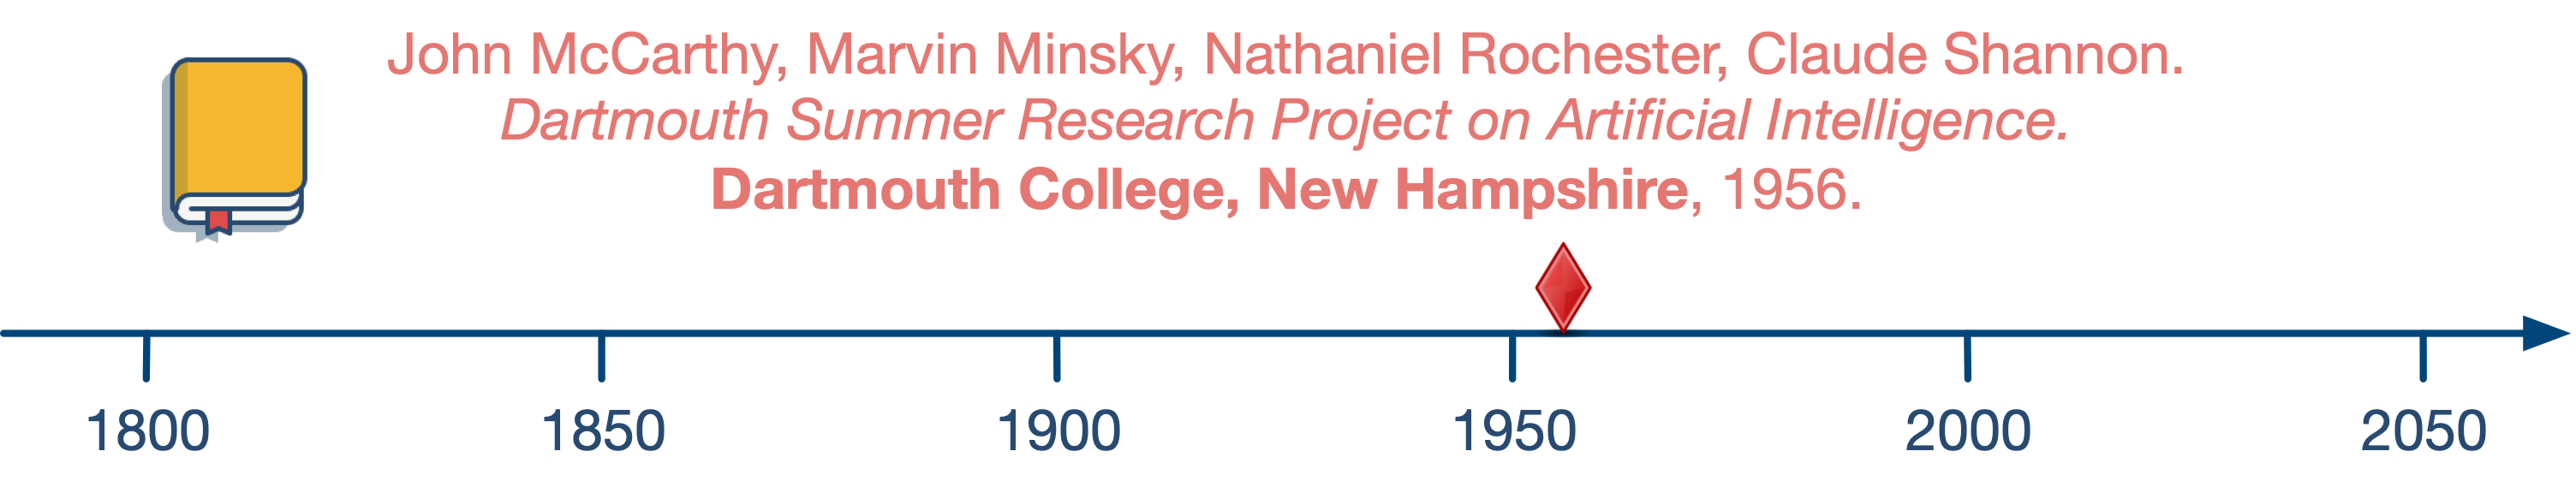
\includegraphics[width=\textwidth]{img/AI-timeline-1956-2-alt.png}
			\end{figure}
		\end{minipage}
	\onslide<1->
	\begin{minipage}[t]{.4\textwidth}
		\vspace*{10pt}
		\begin{minipage}[t]{0.45\textwidth}
			\centering
			\begin{figure}[ht]
				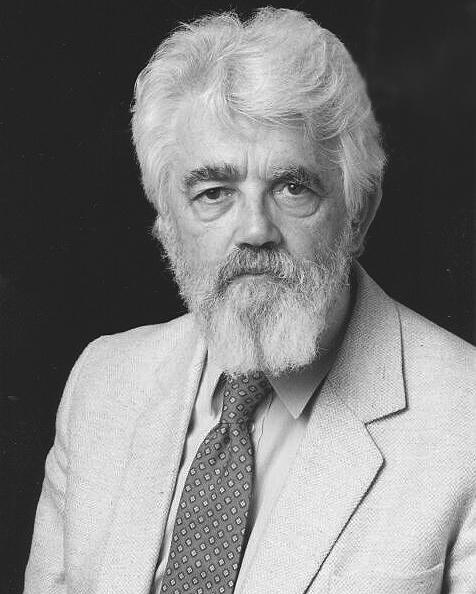
\includegraphics[width=.73\textwidth]{img/John-McCarthy.jpg}
				{\tiny\\John McCarthy\\\vspace*{-1pt}\textit{\textcopyright Naukas}}
			\end{figure}
		\end{minipage}
		\hfill
		\begin{minipage}[t]{0.45\textwidth}
			\centering
			\begin{figure}[ht]
				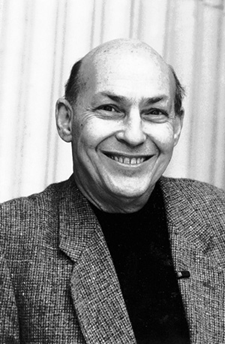
\includegraphics[width=.6\textwidth]{img/Marvin-Misky.png}
				{\tiny\\Marvin Minsky\\\vspace*{-1pt}\textit{\textcopyright Donna Coveny}}
			\end{figure}
		\end{minipage}
		\begin{minipage}[t]{0.45\textwidth}
			\centering
			\begin{figure}[ht]
				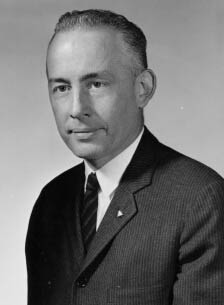
\includegraphics[width=.68\textwidth]{img/Nathaniel-Rochester.jpeg}
				{\tiny\\Nathaniel Rochester\\\vspace*{-1pt}\textit{\textcopyright dmodha}}
			\end{figure}
		\end{minipage}
		\hfill
		\begin{minipage}[t]{0.45\textwidth}
			\centering
			\begin{figure}[ht]
				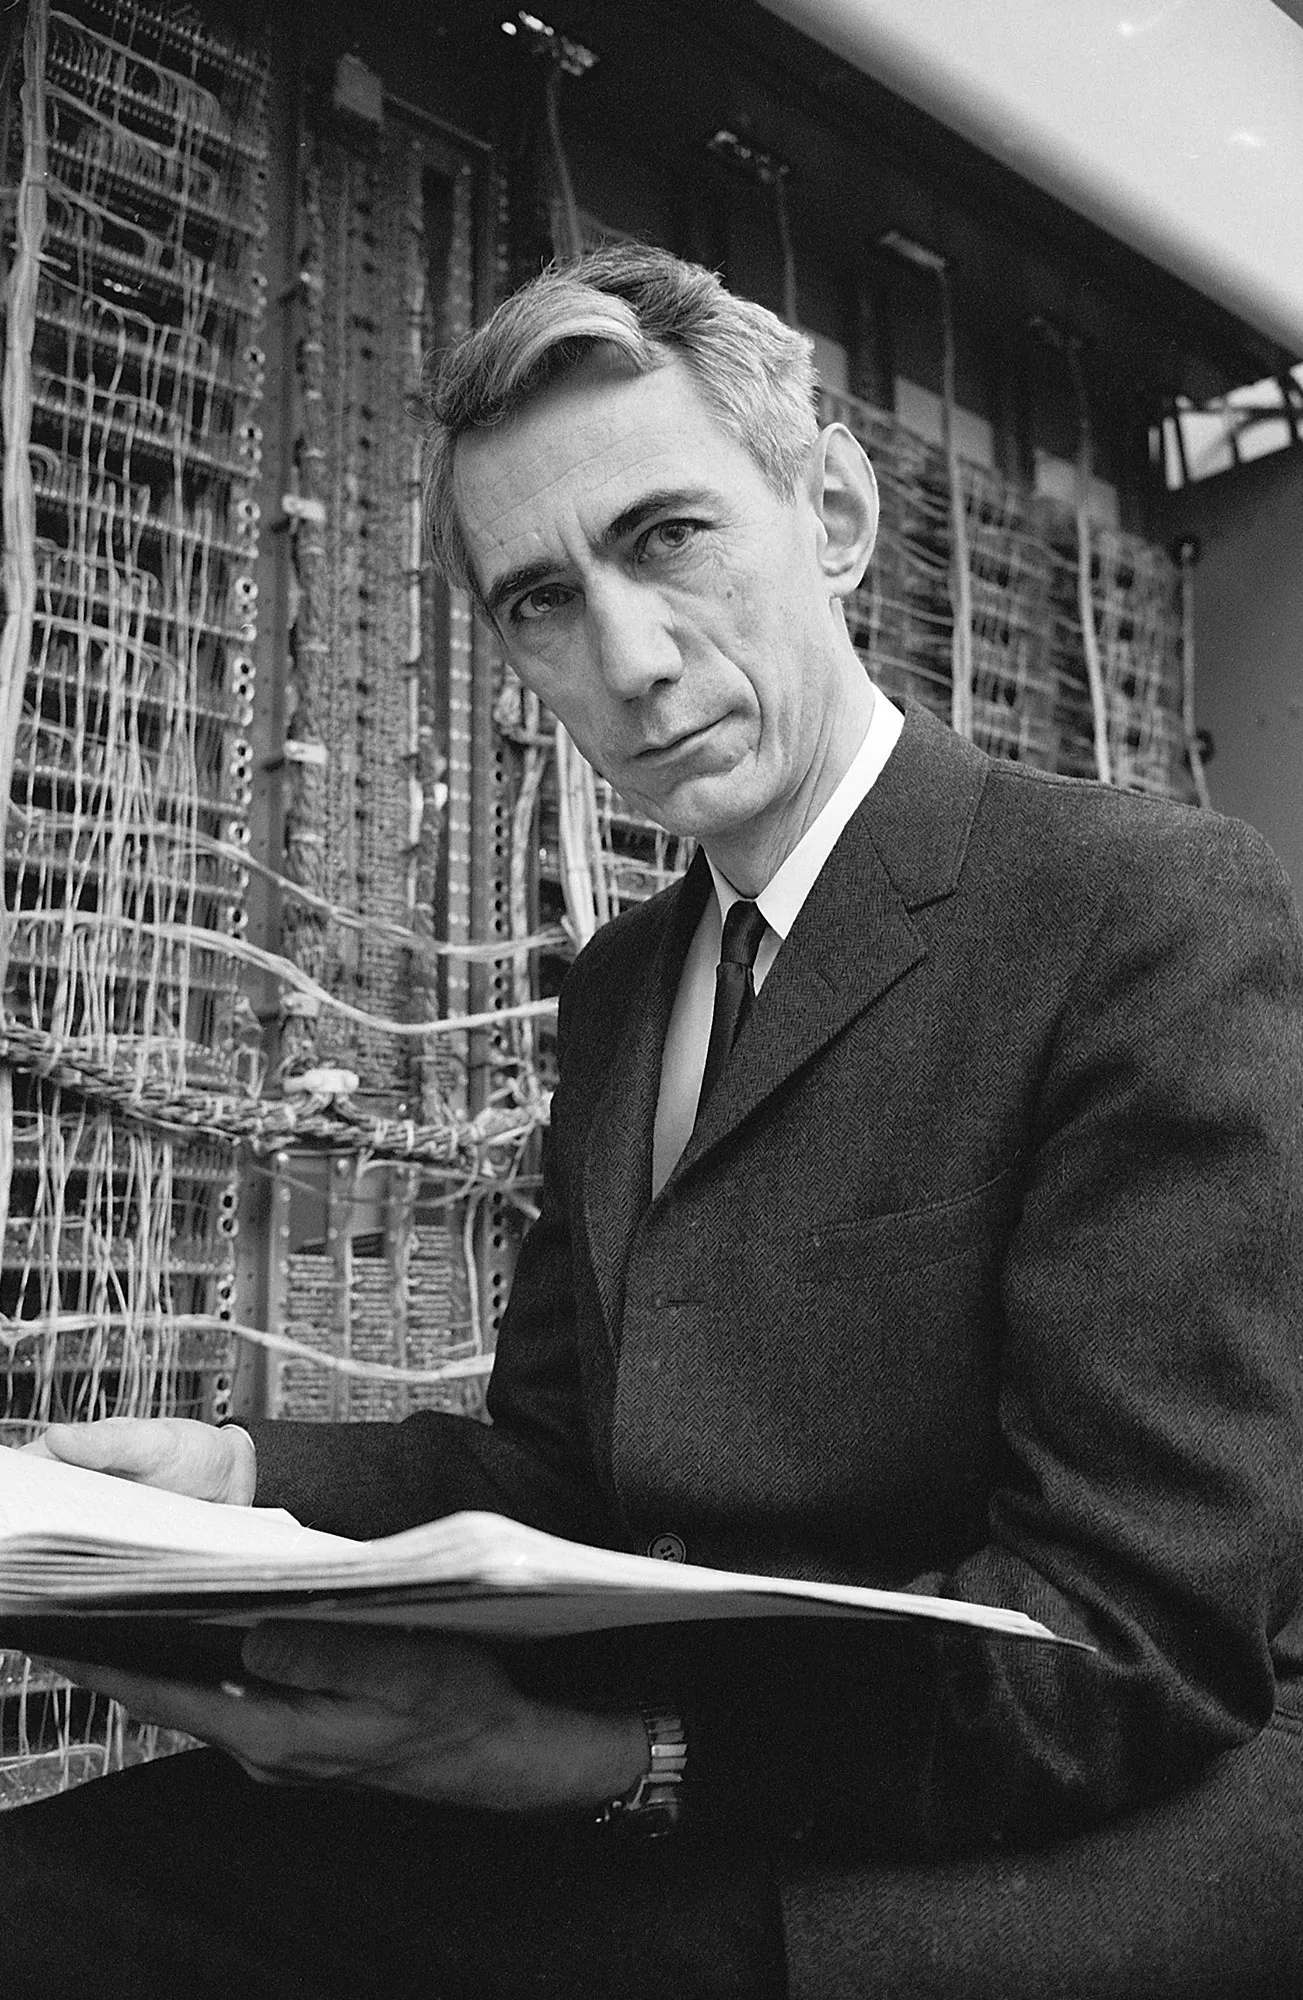
\includegraphics[width=.6\textwidth]{img/Roberts-Claude-Shannon.png}
				{\tiny\\Claude Shannon\\\vspace*{-1pt}\textit{\textcopyright Alfred Eisenstaedt}}
			\end{figure}
		\end{minipage}
	\end{minipage}
	\hfill
	\begin{minipage}[t]{.55\textwidth}
		\renewcommand{\epigraphsize}{\scriptsize}
		\setlength{\afterepigraphskip}{0pt}
		\setlength{\beforeepigraphskip}{10pt}
		\setlength{\epigraphwidth}{\textwidth}
		\epigraph{\textit{Proponiamo che uno studio di 2 mesi, condotto da 10 persone, sull'\alert{intelligenza artificiale} venga svolto durante l'estate del 1956 presso il Dartmouth College di Hanover, nel New Hampshire. Lo studio dovrà procedere sulla base dell'ipotesi che ogni aspetto dell'apprendimento o qualunque altra caratteristica dell'intelligenza possa, in linea di principio, essere descritto con tanta precisione da consentire la costruzione di una macchina capace di simularlo. Si tenterà di scoprire come far sì che le macchine usino il linguaggio, formino astrazioni e concetti, risolvano tipi di problemi attualmente riservati agli esseri umani e siano in grado di migliorare se stesse. [\ldots]
}}{\textit{Summer School Project}, estratto, \textbf{Dartmouth, 1956}\\Traduzione: \textit{\textcopyright ChatGPT}}
	\end{minipage}%
	}
\end{frame}
%
\begin{frame}[t,fragile] \frametitle{Cronistoria della AI}
	\only<1>{\framesubtitle{1950-1975: dalle stelle\ldots}}
	\vspace*{-15pt}
	\only<1>{
    	\begin{figure}[ht]
        	\centering
        	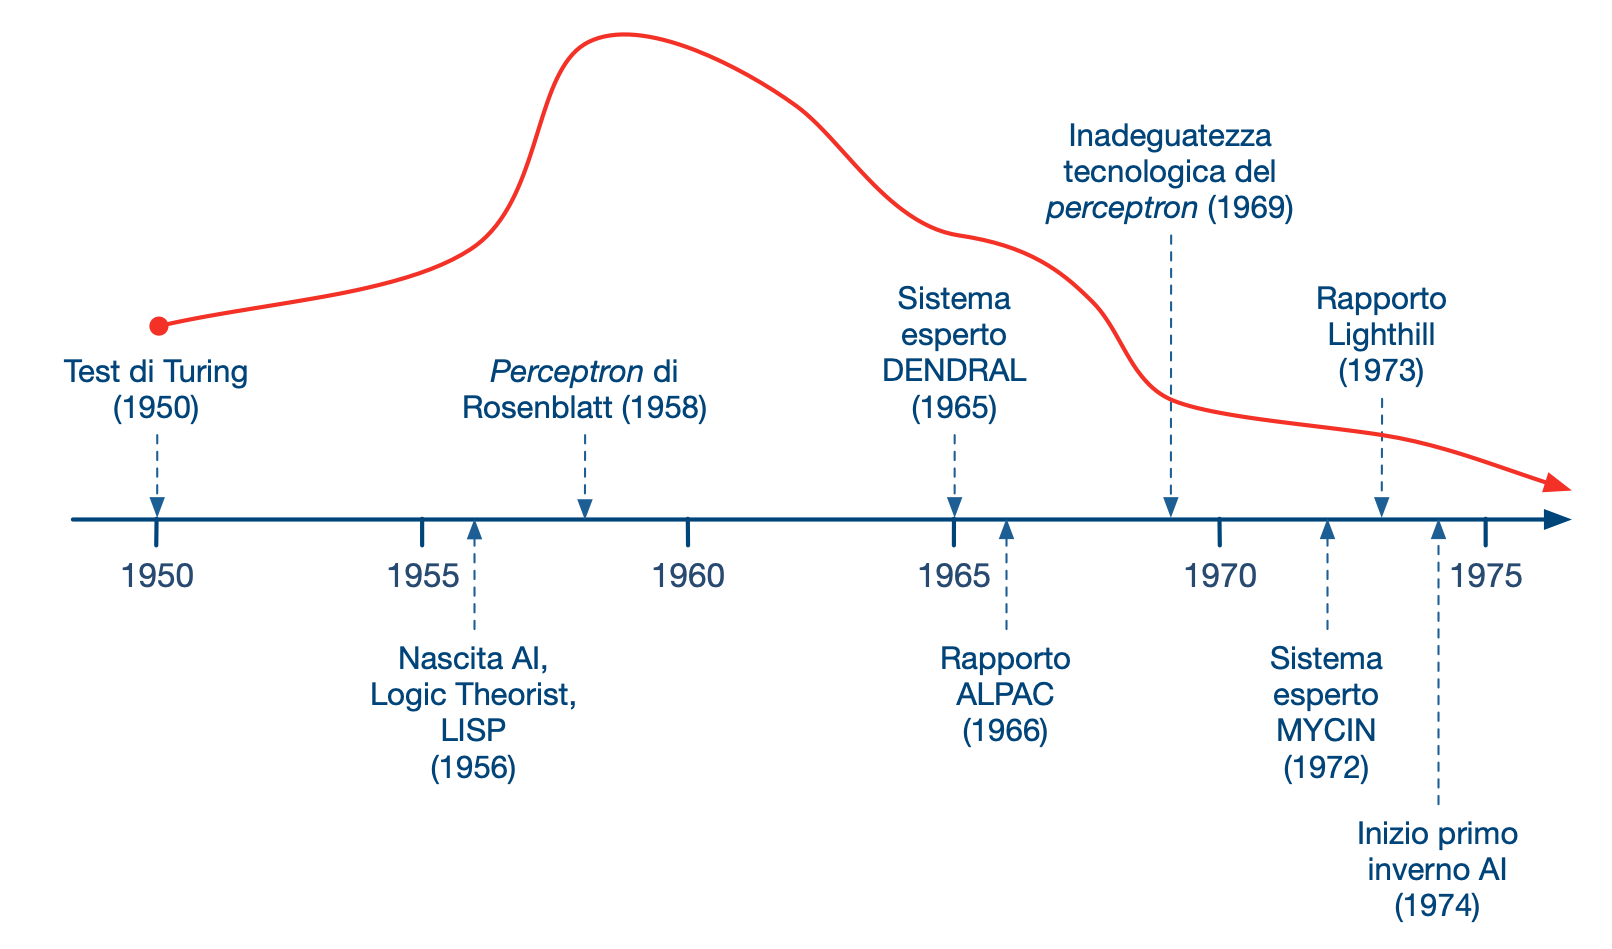
\includegraphics[width=\textwidth]{img/AI-rollercoaster-1.png}
    	\end{figure}
	}
	\begin{flushright}
    	\vspace*{-10pt}
        {\tiny\textit{\textcopyright Simone Scannapieco. I valori delle ordinate sono puramente indicativi.}}
	\end{flushright}
\end{frame}
%
\begin{frame}[t,fragile] \frametitle{Cronistoria della AI}
	\framesubtitle{1950-1975: cause del primo inverno AI}
	{\small
	\begin{itemize}[leftmargin=10pt,align=right]
	\only<1>{\item[\alert{\faHandORight}] \alert{Aspettative esagerate:} la ricerca in IA fece previsioni troppo audaci sulle capacità dell'IA che non si sono materializzate (Rosenblatt, 1958)}
	\only<2>{\item[\alert{\faHandORight}] \alert{Limitazioni tecniche:} potenza di calcolo e algoritmi insufficienti per risolvere problemi complessi del mondo reale (\textit{perceptron})}
	\end{itemize}
	\only<1>{
	\begin{minipage}[t]{\textwidth}
		\begin{minipage}[t]{\textwidth}
			\begin{minipage}[t]{.32\textwidth}
				\renewcommand{\epigraphsize}{\scriptsize}
				\setlength{\afterepigraphskip}{0pt}
				\setlength{\beforeepigraphskip}{5pt}
				\setlength{\epigraphwidth}{0.9\textwidth}
				\epigraph{\textit{[$\ldots$] stiamo per assistere alla nascita di una macchina [$\ldots$] capace di percepire, riconoscere e identificare ciò che la circonda senza alcun addestramento o controllo da parte dell'essere umano.}}{F. Rosenblatt, Mark I Perceptron, 1958}
			\end{minipage}%
			\begin{minipage}[t]{.32\textwidth}
				\renewcommand{\epigraphsize}{\scriptsize}
				\setlength{\afterepigraphskip}{0pt}
				\setlength{\beforeepigraphskip}{5pt}
				\setlength{\epigraphwidth}{0.9\textwidth}
				\epigraph{\textit{[$\ldots$] è il primo rivale del cervello umano che sia mai stato concepito.}}{New Yorker, 1958}
			\end{minipage}%
			\begin{minipage}[t]{.32\textwidth}
				\renewcommand{\epigraphsize}{\scriptsize}
				\setlength{\afterepigraphskip}{0pt}
				\setlength{\beforeepigraphskip}{5pt}
				\setlength{\epigraphwidth}{0.9\textwidth}
				\epigraph{\textit{Ecco il cervello elettronico che insegna a se stesso.}}{The New York Times, 1958}
			\end{minipage}%
		\end{minipage}
	\end{minipage}
	}
	\only<2>{
	\begin{minipage}[t]{\textwidth}
		\begin{minipage}[t]{0.6\textwidth}
			\centering
			\begin{figure}[ht]
				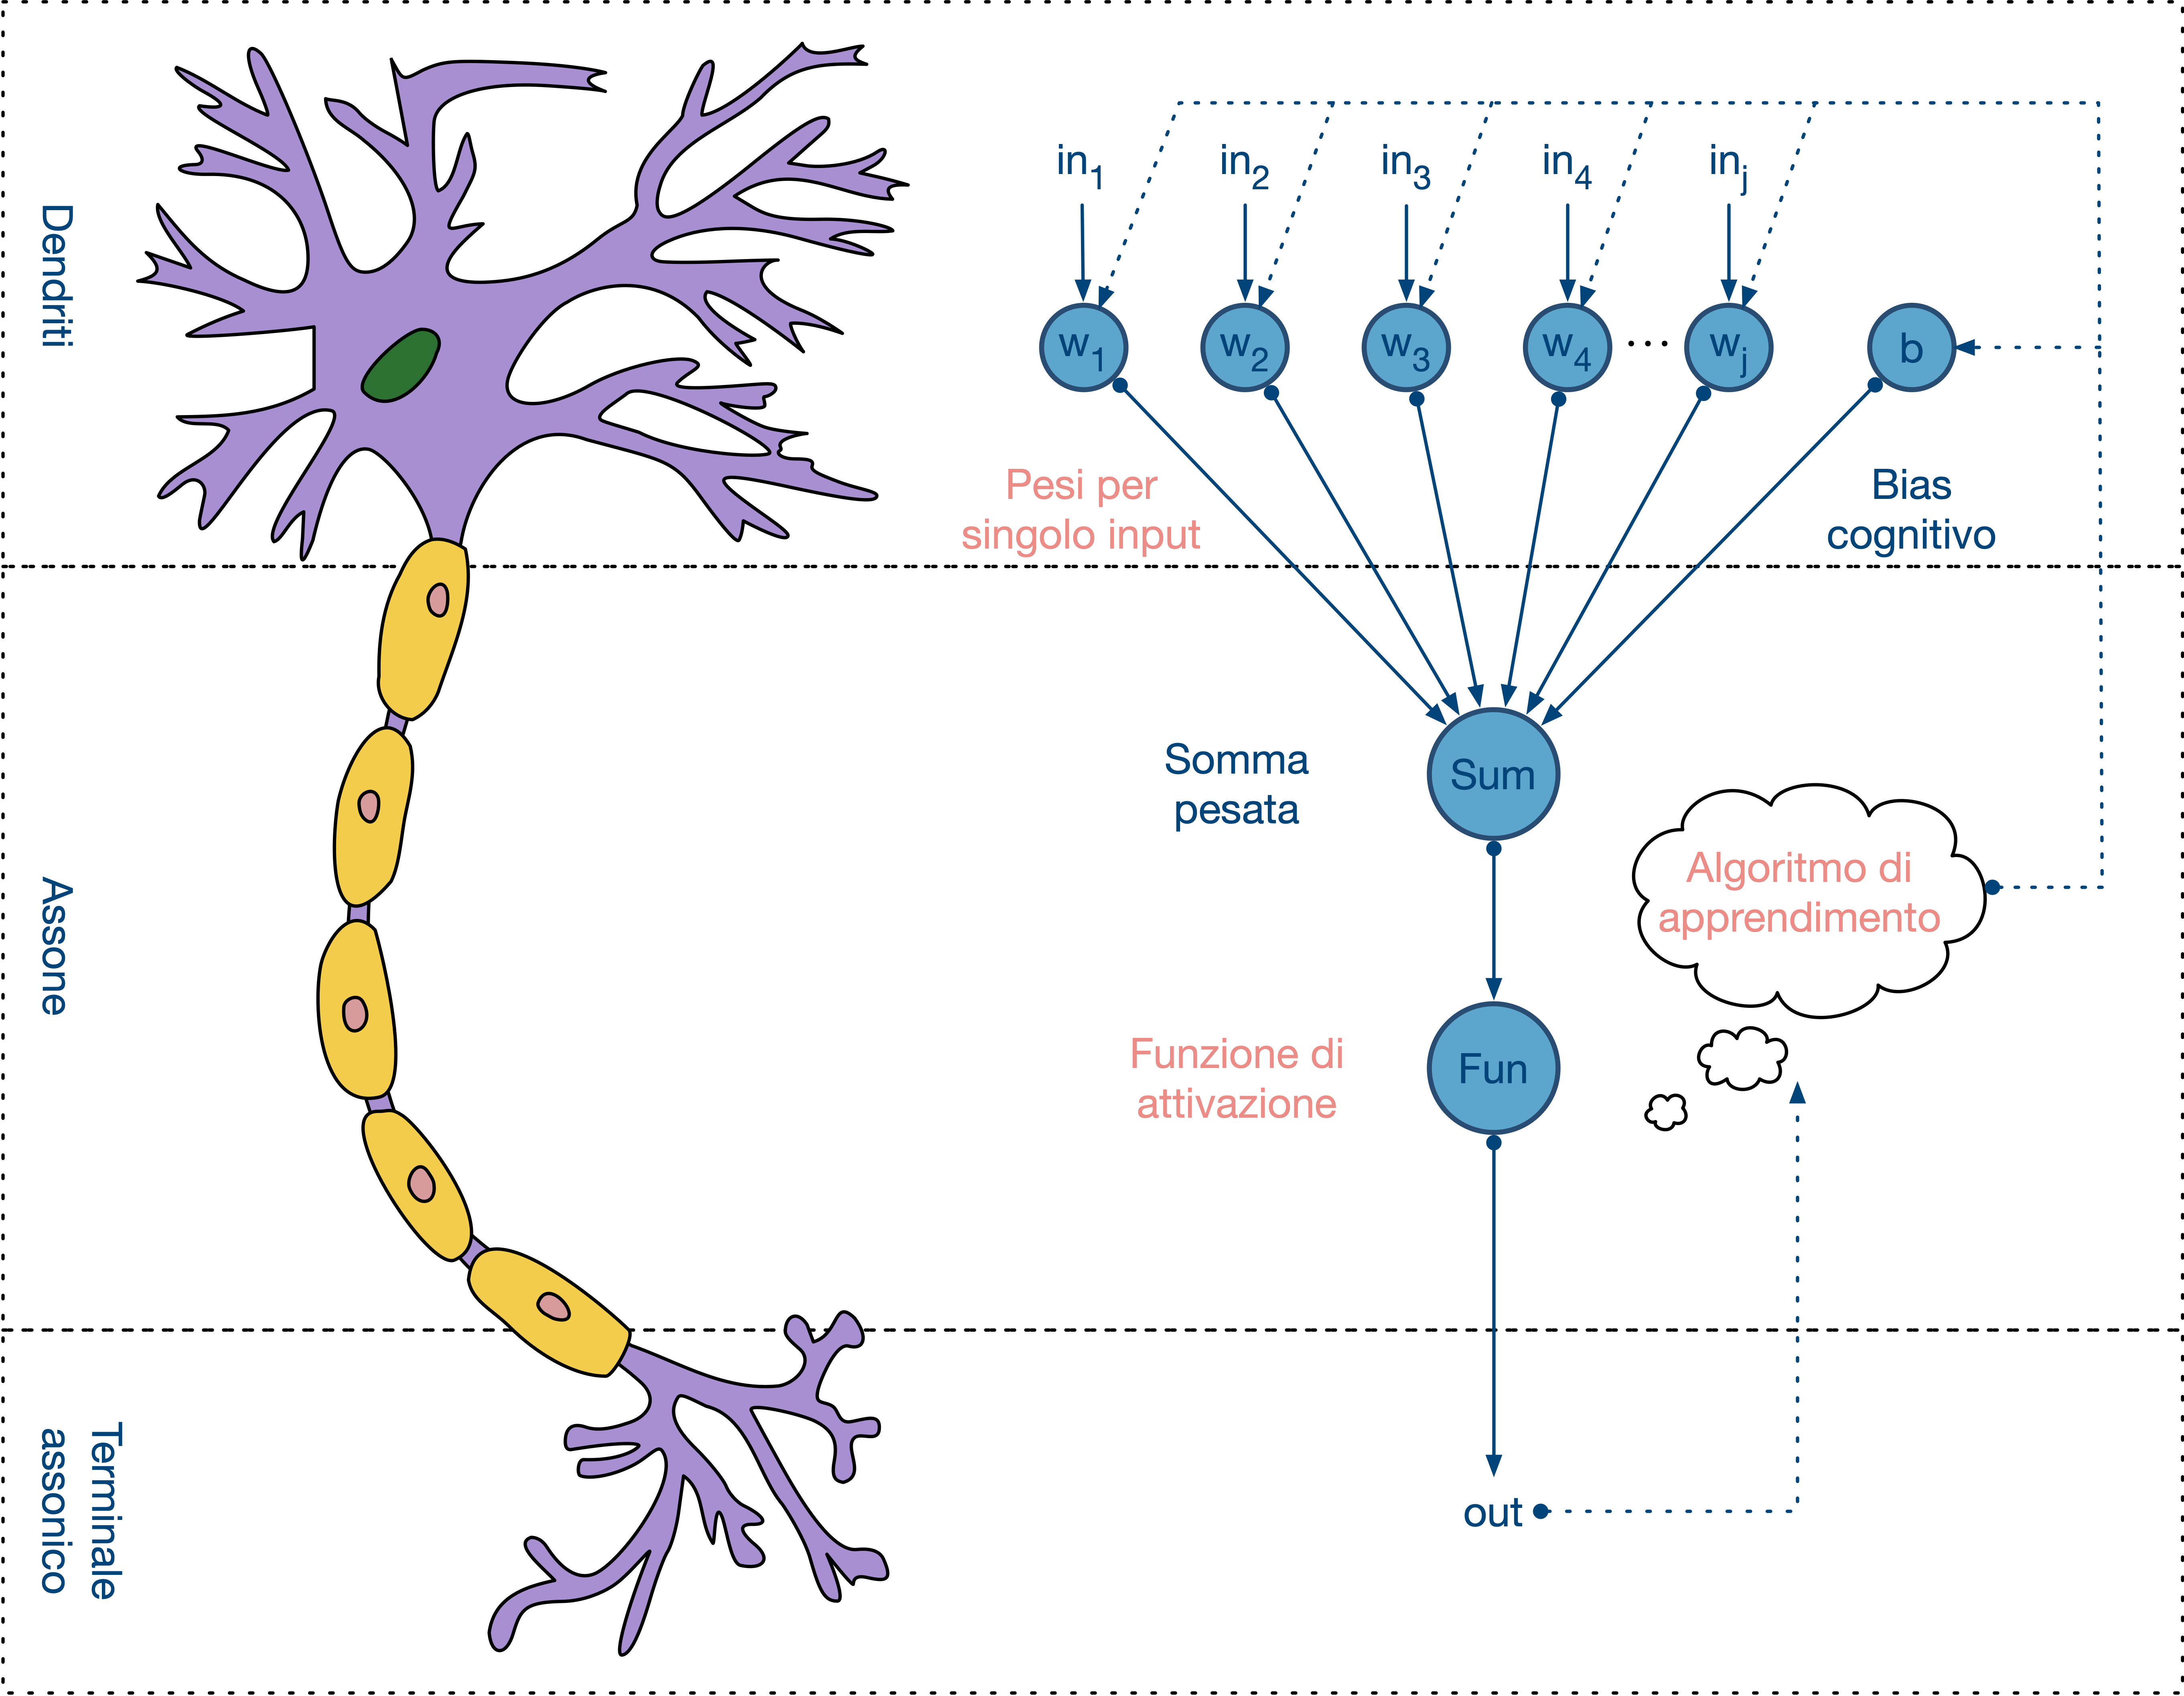
\includegraphics[width=.8\textwidth]{img/Perceptron-vs-neuronal-cell.png}
				{\tiny\\Neurone umano vs. \textit{perceptron}\\\vspace*{-4pt}\textit{\textcopyright Simone Scannapieco, Wikimedia Creative Commons}}
			\end{figure}
		\end{minipage}
		\onslide<1->
		\begin{minipage}[t]{0.4\textwidth}
			\centering
			\begin{figure}[ht]
				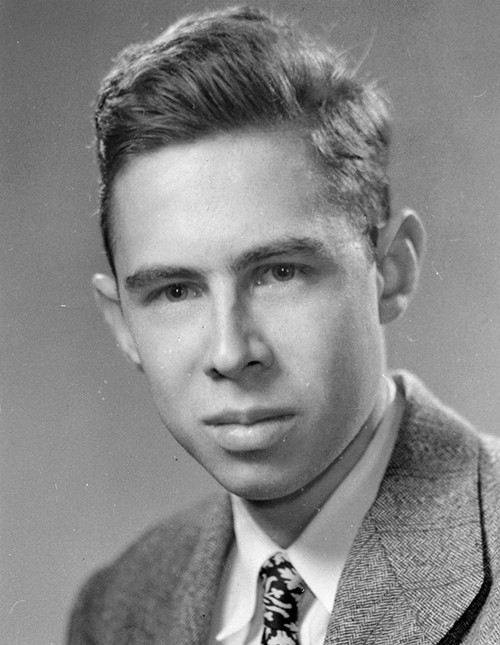
\includegraphics[width=.61\textwidth]{img/Frank-Rosenblatt.jpg}
				{\tiny\\Frank Rosenblatt\\\vspace*{-4pt}\textit{\textcopyright Wikimedia Creative Commons}}
			\end{figure}
		\end{minipage}
	\end{minipage}
	}
	}
\end{frame}
%
\begin{frame}[t,fragile] \frametitle{Cronistoria della AI}
	\only<1>{\framesubtitle{1975-2000: \ldots di nuovo alle stelle}}
	\vspace*{-15pt}
	\only<1>{
    	\begin{figure}[ht]
        	\centering
        	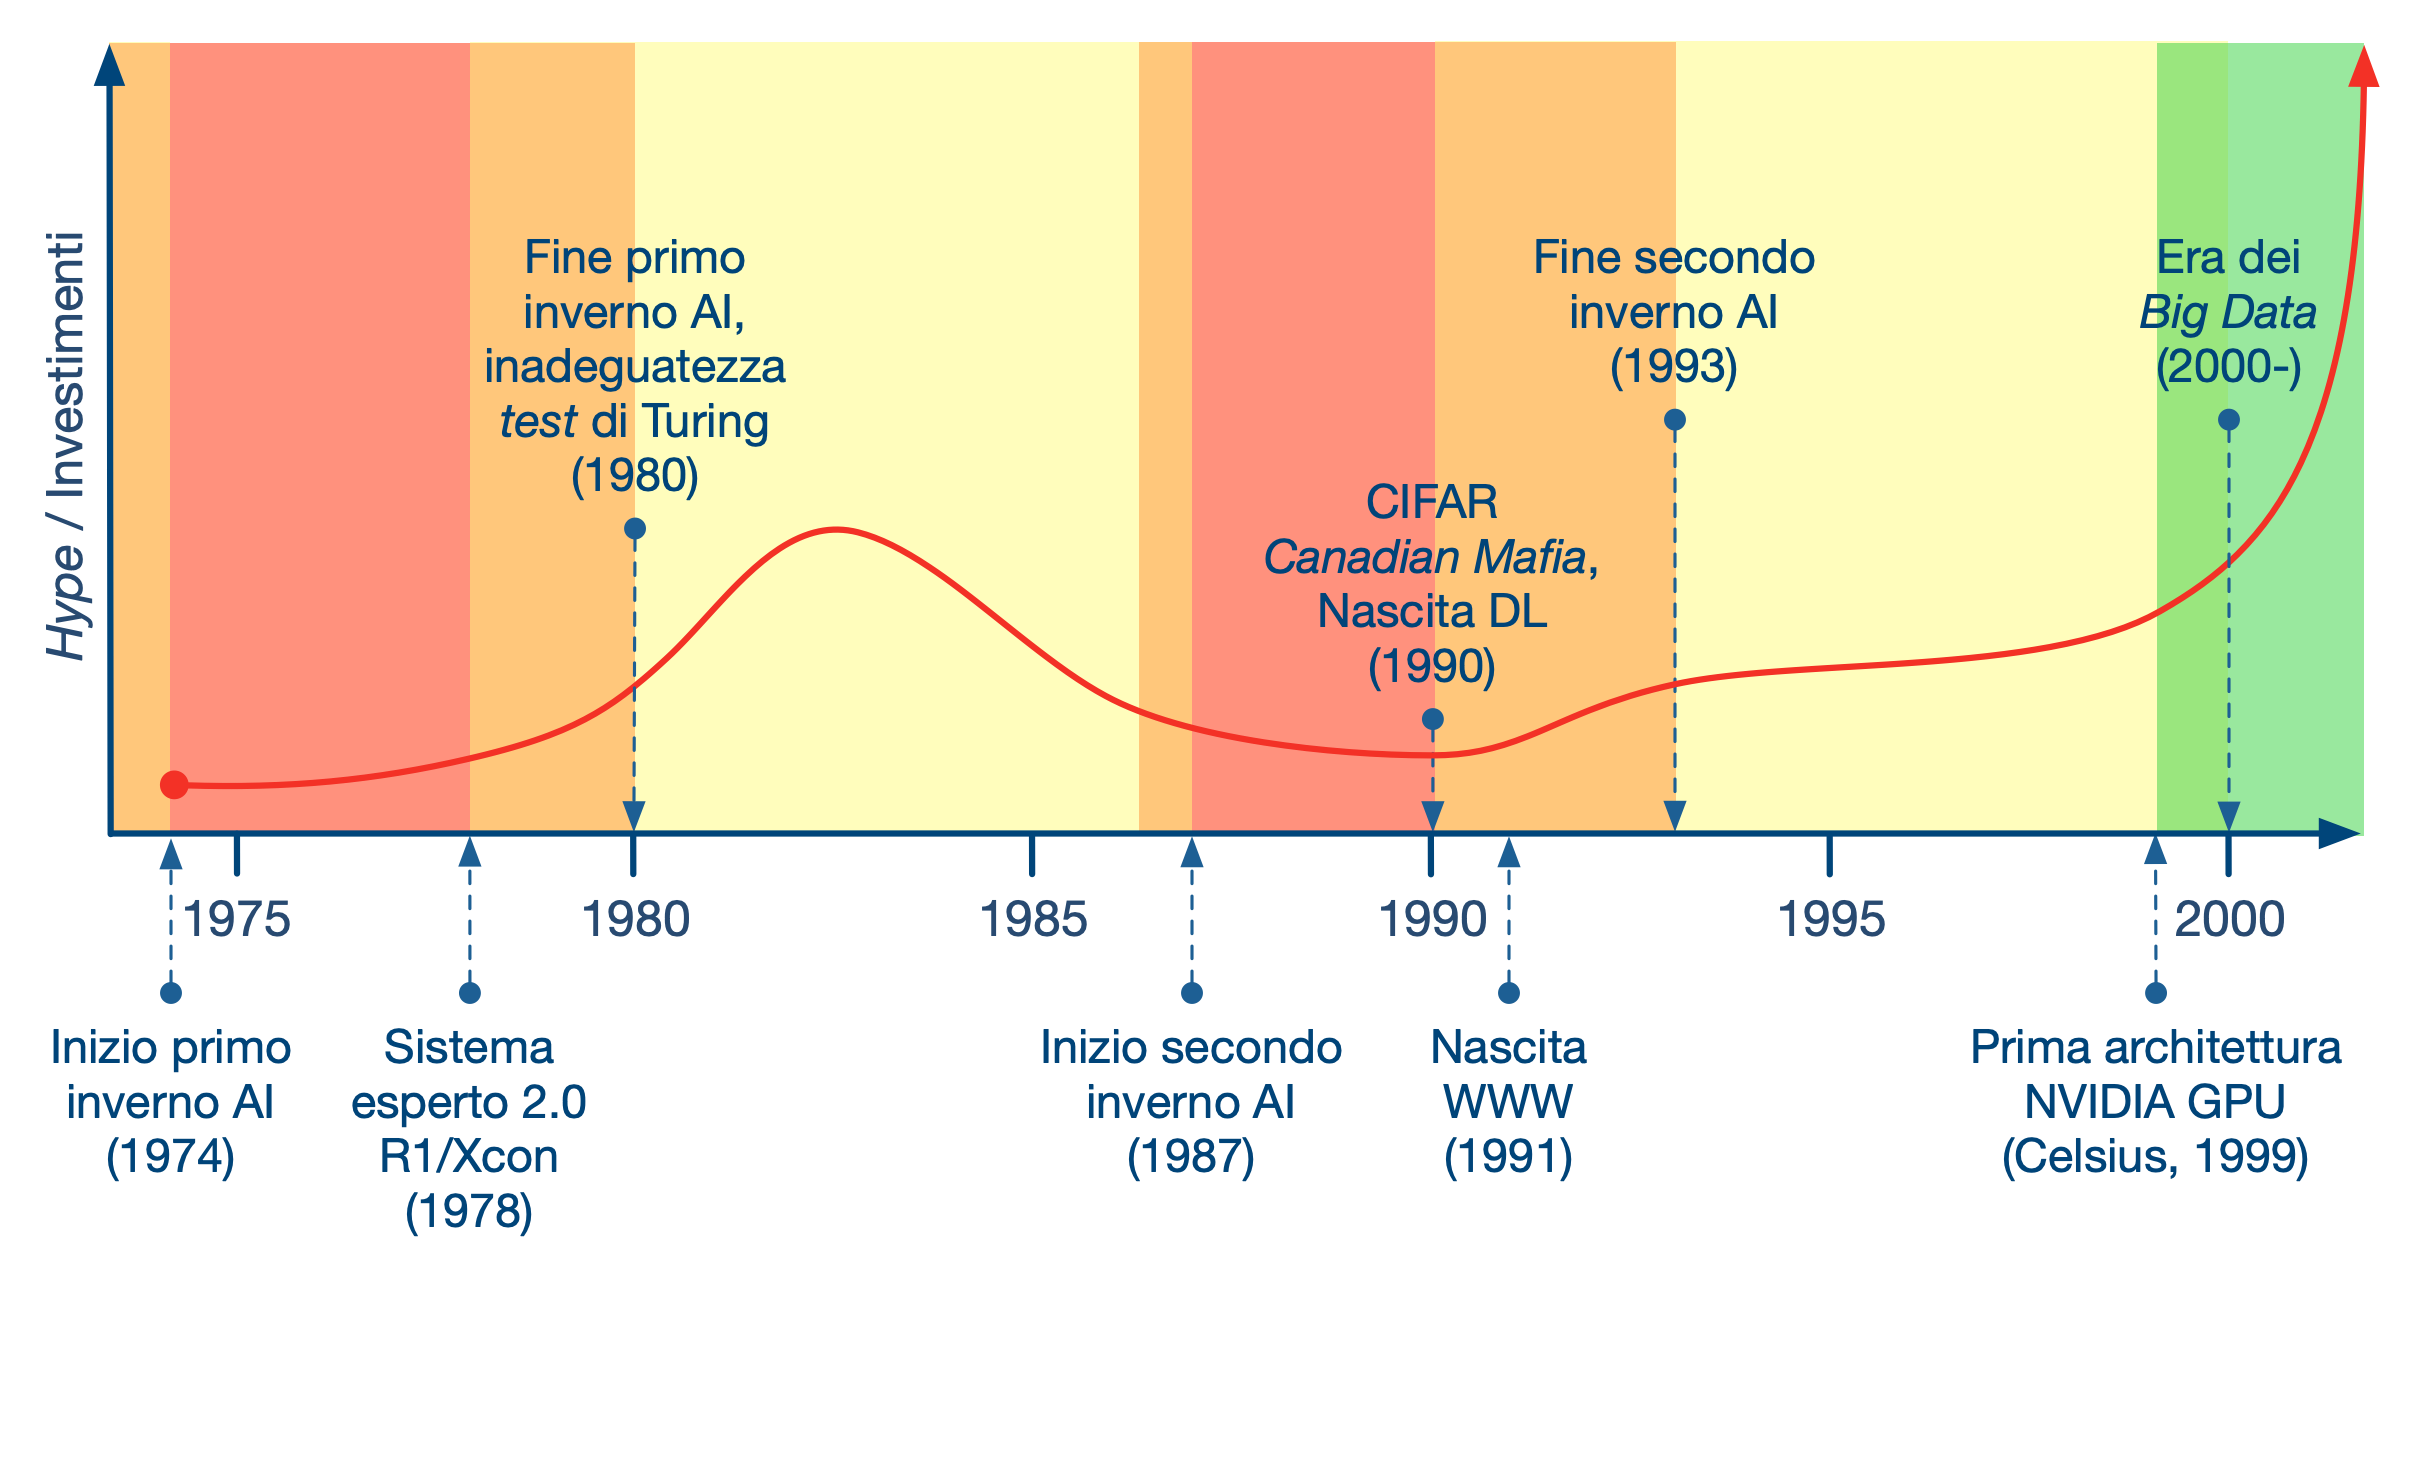
\includegraphics[width=\textwidth]{img/AI-rollercoaster-2.png}
    	\end{figure}
	}
	\begin{flushright}
    	\vspace*{-10pt}
        {\tiny\textit{\textcopyright Simone Scannapieco. I valori delle ordinate sono puramente indicativi.}}
	\end{flushright}
\end{frame}
%
\begin{frame}[t,fragile] \frametitle{Cronistoria della AI}
	\only<1>{\framesubtitle{1975-2000: fattori di ripresa}}

\end{frame}
%
\begin{frame}[t,fragile] \frametitle{Intelligenza Artificiale}
{\scriptsize
	\onslide<1->
		\framesubtitle{Secondo il creatore della AI}
		\vspace*{3pt}
		\begin{minipage}[t]{\textwidth}
			\begin{minipage}[t]{0.45\textwidth}
				\centering
				\begin{figure}[ht]
					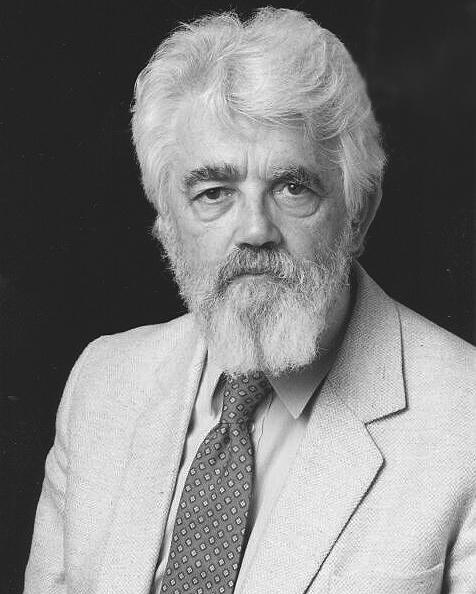
\includegraphics[width=.73\textwidth]{img/John-McCarthy.jpg}
					{\tiny\\John McCarthy\\\vspace*{-1pt}\textit{\textcopyright Naukas}}
				\end{figure}
			\end{minipage}
		    \begin{minipage}[t]{0.5\textwidth}
				\renewcommand{\epigraphsize}{\small}
				\setlength{\afterepigraphskip}{0pt}
				\setlength{\beforeepigraphskip}{5pt}
				\setlength{\epigraphwidth}{\textwidth}
				\epigraph{
					\textit{\alert{D:} Cosa è l'Intelligenza Artificiale?\\
					\alert{R:} E' la scienza e l'ingegneria di creare macchine intelligenti, in particolare programmi informatici intelligenti. È correlata al compito simile di utilizzare i computer per comprendere l'intelligenza umana, ma l'intelligenza artificiale non deve limitarsi a metodi che siano osservabili biologicamente.}}{John McCarthy, \textbf{Stanford Uni, 2007}\\Traduzione: \textit{\textcopyright ChatGPT}}
			\end{minipage}
		\end{minipage}
}
	\onslide<2->
	\begin{itemize}[leftmargin=10pt,align=right]
		\item[\alert{\faHandORight}] Sistema di AI è un termine estremamente inflazionato\ldots 
		\onslide<3->\item[\alert{\faHandORight}] \ldots anche per sistemi che AI non sono affatto
	\end{itemize}
\end{frame}
%
\begin{frame}[t,fragile] \frametitle{NON Intelligenza Artificiale}
	\vspace*{-15pt}
	\begin{center}
		\begin{minipage}[t]{0.6\textwidth}
			\centering
			\begin{figure}[ht]
				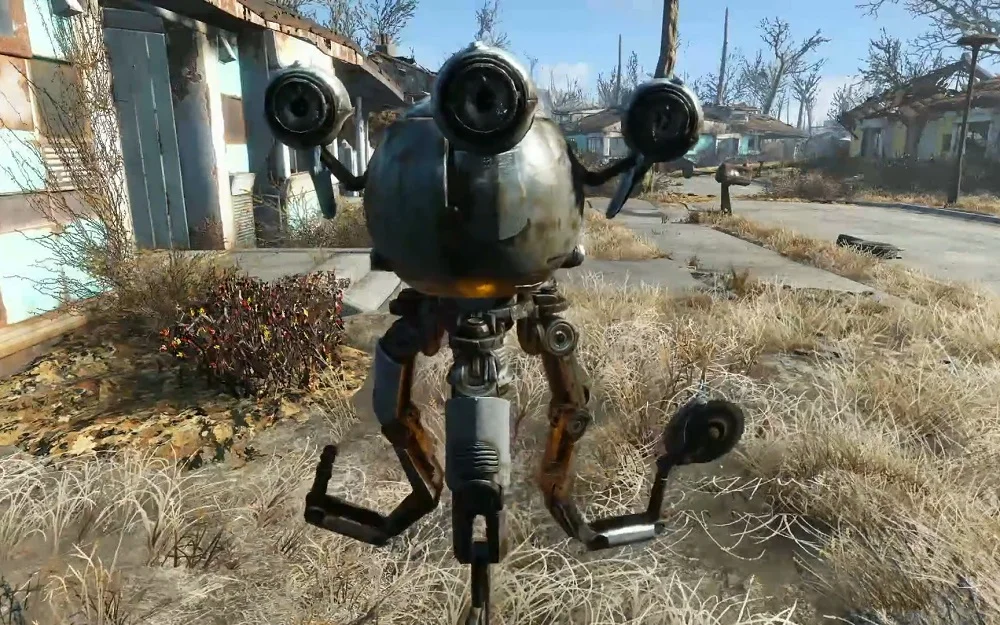
\includegraphics[width=\textwidth]{img/codsworth.png}
			\end{figure}
		\end{minipage}
		\begin{minipage}[t]{.6\textwidth}
			\renewcommand{\epigraphsize}{\tiny}
			\setlength{\afterepigraphskip}{0pt}
			\setlength{\beforeepigraphskip}{5pt}
			\setlength{\epigraphwidth}{\textwidth}
			\epigraph{\textit{Questo significa che sei, ehm\ldots in ritardo di due secoli per cena! Forse potrei prepararti uno spuntino? Devi essere affamato!}}{Codsworth all'Unico Sopravissuto, \textbf{Fallout 4, 2015}\\\vspace*{0pt}\textit{\textcopyright Nukapedia: The Fallout Wiki}}
		\end{minipage}
	\end{center}
	\onslide<2->
	\begin{itemize}[leftmargin=10pt,align=right]
		\item[\alert{\faHandORight}] \alert{\textit{Non-Playable Characters}} (NPC) dei \textit{videogame} 
		\onslide<3->\item[\alert{\faHandORight}] Sistemi di regole \textit{if-then-else}, \alert{non} AI
	\end{itemize}
\end{frame}